\chapter{Durchf\"uhrung der Messungen}

\section{Vorbereitung und Kalibrierung}
\subsection{Funktions\"uberpr\"ufung (L\"otstellen und Testboard) \(Bellgardt, Menzel\)}


\subsection{Externe Shunt Kalibrierung (graues Ger\"at und Rechnung) \(Nerb, Ulit\)}
%\subsection{Geometrische Kalibrierung (Biegebalken und Rechnung) (UN)}

\section{Messungen am Fahrradlenker \(Bellgardt, Menzel\)}
\subsection{Aufbau Testvorrichtung}
\subsection{Durchf\"uhrung Messung (Kraft, Konzept, Vertikal/Horizontal)}

\clearpage
\section{Messungen am Flying Suit (Fluggestell) \(Nerb, Ulit\)}
\subsection{Kurzbeschreibung Flying Suit}
Der „FlyingSuit“ ist eine Entwicklung des Tüftlers Konstantin Landuris und seines Künstlerstudios „Landurisstudios“.
Es handelt sich dabei um die Idee, ein Jetpack mit elektrischen Antrieben zu versehen und den Transport einer Person zu ermöglichen.

\begin{figure}[htbp]
    \centering
    \begin{minipage}{0.48\textwidth}
        \centering
        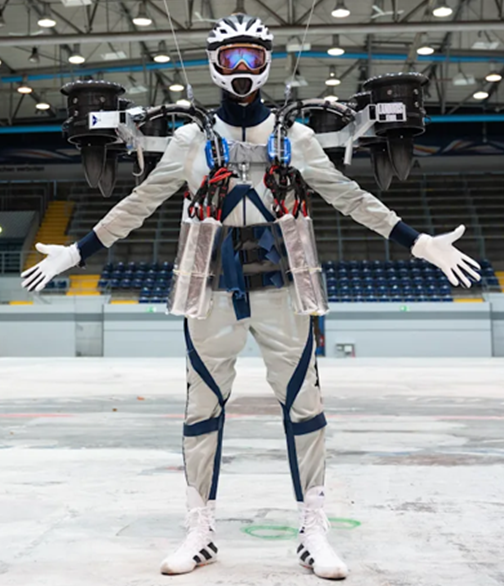
\includegraphics[width=\textwidth]{lan1.png}
        \caption[Flying Suit Landuris (Abbildungsverzeichnis)]{Flying Suit Landuris}
        \cite{Landuris}
        \label{fig:lan1}
    \end{minipage}
    \hfill
    \begin{minipage}{0.48\textwidth}
        \centering
        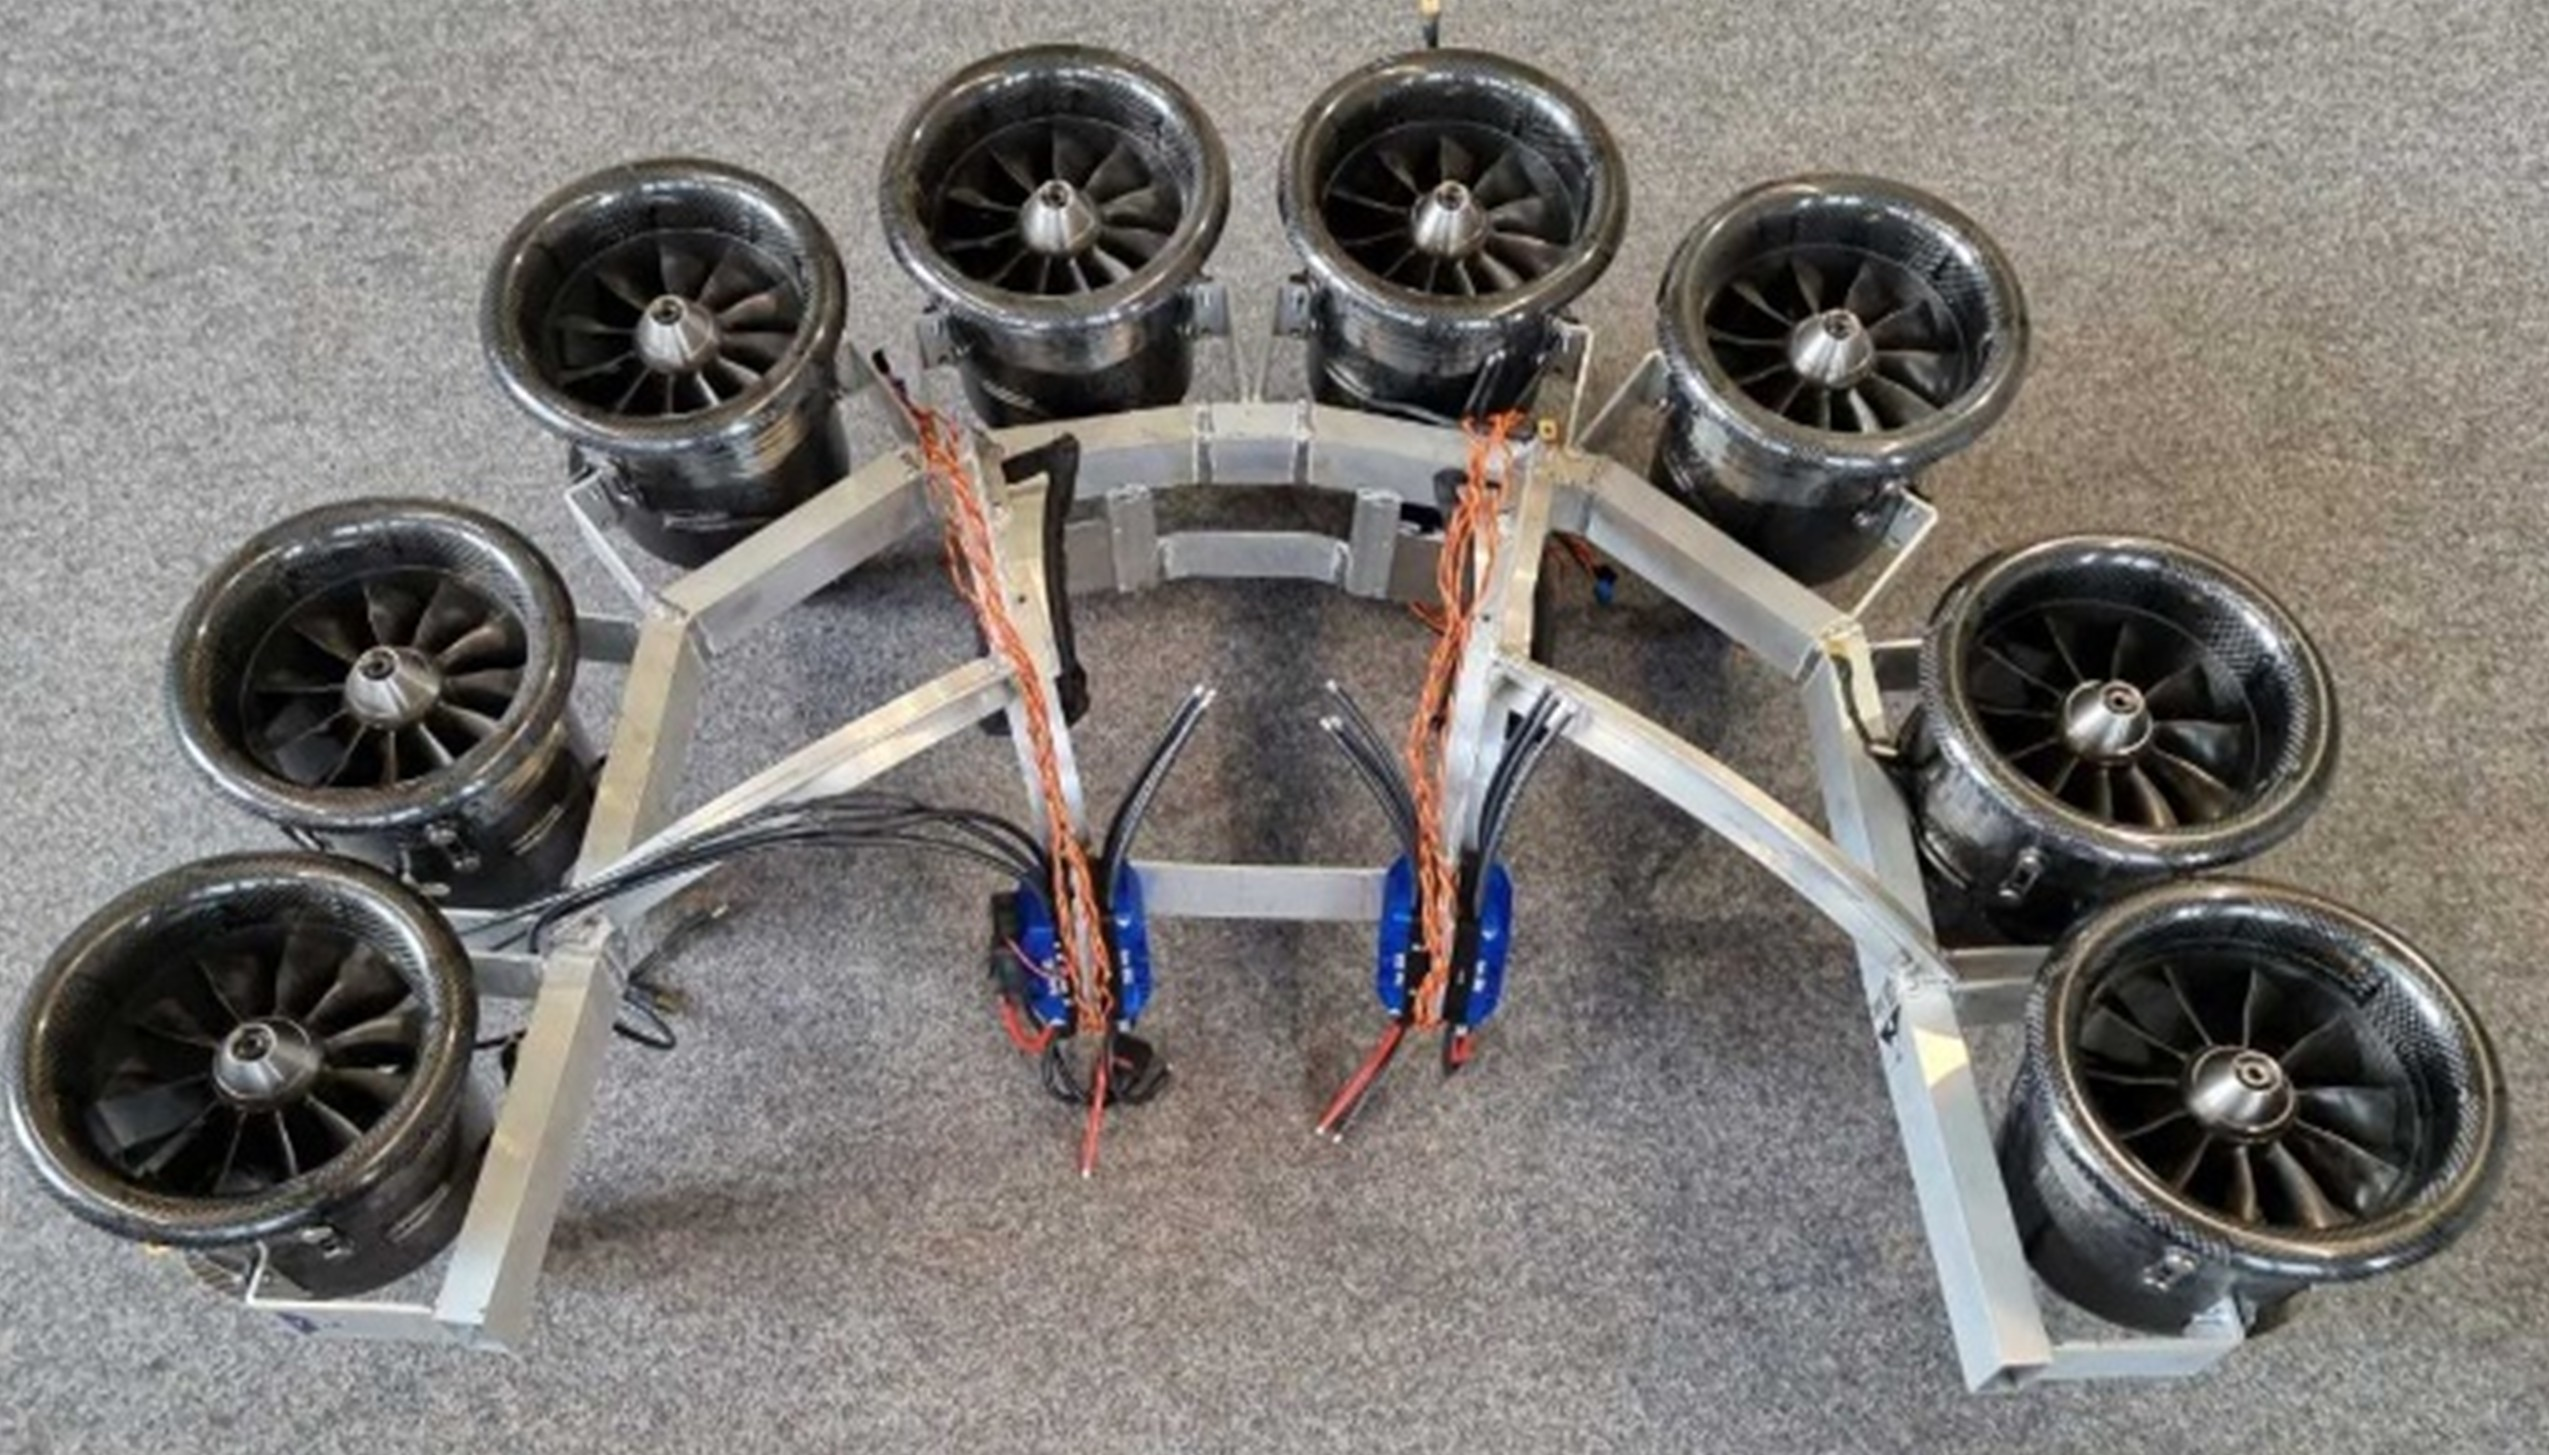
\includegraphics[width=\textwidth]{lan2.jpg}
        \caption[Flying Suit Gestell (Abbildungsverzeichnis)]{Flying Suit Gestell}
        \cite{Landuris}

        \label{fig:lan2}
    \end{minipage}
\end{figure}

Durch den Verzicht auf klassische Triebwerke, soll langfristig die Sicherheit, die Effizienz, Umweltbelastung und auch Lärmverursachung deutlich verbessert werden.
Der Anzug besteht dabei grundsätzlich aus zwei Teilen, einem reißfesten Overall mit eingearbeiteten Gurten zur Kraftverteilung und Stabilisierung des Systems,
sowie einem auf den Schultern gestützten Gestell, an welchen die Triebwerke montiert sind. Lenkbewegungen erfolgen dabei primär über die Verlagerung des Körpergewichts,
sodass die Hände zunächst zur Schubregelung und in einem fortgeschrittenen Stadium auch zur Ausführung von Arbeiten verwendet werden könnten.
Die eingearbeiteten Gurte führen von den Füßen, über den Körper, bis mittig zu Brust und Rücken, wo je eine Fassung zur Aufnahme von Karabinerhaken o.Ä. befestigt ist.
Über diese beiden Punkte ist der Overall mit dem Gestell verbunden und übertragene Kräfte werden hier eingeleitet. Benötigte Akkus werden am Körper befestigt mitgeführt. 
Bei dem zur Vermessung Vorliegendem Modell, handelt es sich um den ersten entwickelten Prototypen.
Dieser besteht aus geschweißten, hohlen Aluminium-Rechteck Trägern mit den Profilmaßen h= 50mm x b= 45mm, Wandstärke= 2mm.
Zudem sind Tragebügel an den Schultern, sowie im Brustbereich und Querstreben zur Versteifung vorhanden.
Die Abmaße belaufen sich, ohne Triebwerke, auf 96cm in der Breite und 67cm in der Tiefe. Das Gewicht beläuft sich auf 8,4Kg, ebenfalls exklusive Triebwerke.
Hinten und seitlich sind insgesamt acht DS-130-DIA HST® (152 mm) Modellbautriebwerke mit je max. 175N (150N reale Bedingungen) Schubleistung angebracht,
welche in ersten realen Flugversuchen, kurzeitig genügend Auftrieb für einen kurzzeitigen Schwebeflug mit einer Person aufgebracht haben.
Eine stabile und ausgereifte Lagerregelung ist jedoch noch nicht vorhanden.

\subsection{Vorbereitung}
\subsubsection{Beschreibung der Testszenarien}
Im Rahmen des Experimentaltechnik- Projektes liegt der Fokus auf der Entwicklung, der Montage, sowie dem ersten Einsatz eines Messkonzeptes im Zusammenspiel mit dem zuvor im Bericht beschriebenen drahtlosen Datenloggers VLink 200.
Ziel ist es eine erste Möglichkeit zu schaffen, Daten über die wirkenden Kräfte und daraus resultierende Dehnungen und Verformungen zu gewinnen.
Dies soll den Weg bereiten, umfangreichere Tests vornehmen zu können und somit die Verbesserung, speziell des Gestells, voranzubringen.
Daten, die beispielsweise durch einen realen Flugversuch ermittelt werden, könnten dabei helfen die Computergestützte Entwicklung mit echten Messwerten zu hinterlegen.
Reale Flugversuche erzeugen eine Vielzahl, oft nicht klar trennbare Arten von Belastungen in einem Gestell, wie dem uns vorliegenden.
Aus diesem Grund basieren die folgend erläuterten Testfälle, auf vereinfachten, nicht aber unrealistischen, Annahmen. 
Ausgangspunkt für die Messungen ist zunächst der statische Lastfall oder „Schwebezustand“.
Hierbei gleichen sich alle Kräfte gegenseitig aus, was bedeutet, dass die erzeugten Schubkräfte, sowohl das Gestell, den Piloten, die Akkus mit 8x2Kg und 1Kg Messbox tragen. 

\textbf{Zugkräfte} sollen an den Aufnahmepunkten zwischen Anzug und Gestell bestimmt werden.
Das Ziel dieses Tests ist es, die gleichmäßige Verteilung der Kräfte zwischen vorderer und hinterer Befestigung zu ermitteln.
Dies kann beim ausbalancieren des gesamten Systems helfen, was in einer Flugphase eine ausgewogenere und leichtere Steuerung zur Folge haben kann.
Darüber hinaus können Lasten wie z.B. die Akkus, gleichmäßig angebracht werden. 

\textbf{Biegung} tritt kann an unterschiedlichen Stellen des Messgestells auftreten. Grundsätzlich führt jede Kraft an einem Hebelarm, zu einem Moment.
Die Schubkräfte der Triebwerke, greifen dabei an mehreren Punkten mit verschieden langen Hebelarmen an, was in Abhängigkeit der Länge des Hebels,
sowie Betrag und Richtung der Kraft, zu je einem Beitrag an Biegung führt. Eine Möglichkeit wäre es abschnittsweise von vorne nach hinten zu messen,
wodurch die Biegung je Teilsegment bestimmt werden könnte. Zusätzlich könnte man einen Nutzen der Querversteifungen abschätzen. Darüber hinaus kann man einen Links-rechts-Vergleich, gegebenenfalls auch je Teilsegment vornehmen, was auf ungleichen Schub oder auch Bauteilabweichungen hindeuten kann. In unserem Fall haben wir vereinfacht den Punkt der maximalen Biegung im Gestell bestimmt, welcher im Bild grün markiert ist. An diesem Punkt hinten mittig, wirken von beiden Seiten jeweils vier Triebwerkskräfte, mit den maximalen Hebelarmlängen, nach oben. Beitragend sind je Seite 120mm, 360mm und zweimal 480mm multipliziert mit der Kraft. Aufgrund des angenommenen Kräftegleichgewichtes kann die Modellbildung gleich eines Kragträgers mit halber breite als Hebelarm und vier wirkenden Triebwerken als Kraft Komponente erfolgen. 

\begin{figure}[htbp]
    \begin{center}
        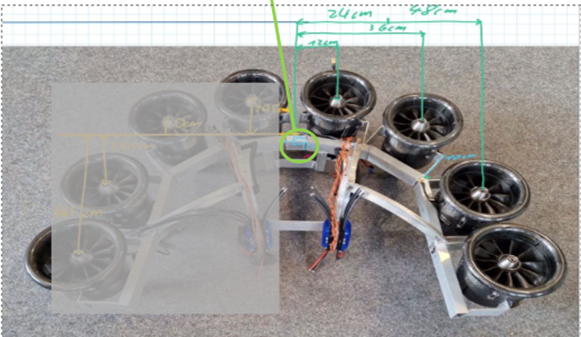
\includegraphics[width=0.75\textwidth, keepaspectratio]{lan3.png}
        \caption[FlyingSuit - wirksame Hebelarme bei der Biegung (Abbildungsverzeichnis)]{FlyingSuit - wirksame Hebelarme bei der Biegung}
        %\footcite{Rechter Teil des Bildes: Praktikum Schwingbruchgefaehrdete Bauteile sicher dimensionieren und betreiben
        %}
        
        \label{fig:lan3}
    \end{center}
\end{figure}


\textbf{Torsion} tritt, analog zur Biegung, häufig nicht in absoluter Reinform auf. Wie bei der Biegung auch sind wirkende Kräfte und Hebelarme,
für entstehende Momente in den Bauteilen verantwortlich. Entscheidend für die Torsion ist die „Verdrehung“ eines Querschnittes,
wodurch maximale Schubspannungen im 45° Winkel verursacht werden, welche wiederum zu einer Schubdehnung führen.
In unserem Fall von Bedeutung sind z.B. die verursachte Torsion der Tragenden Struktur, an welcher parallel die Triebwerke mit einem 100mm Abstand angebracht sind.
Ebenfalls kann hier segmentweise die Torsion betrachtet werden, um auch hier beispielsweise eine Abschätzung für die wirkenden Kräfte oder die Steifigkeit des Gestells vorzunehmen.
Vereinfacht wurde der erdachte maximal Torsionsbelastete Punkt, im Bild grün markiert, ausgesucht.
Ungleiche Triebwerksleistungen oder Bauteilabmessungen der linken und rechten Seite sind ein Grund für auftretende Torsion dort.
Bei einer vereinfachten Annahme, bei welcher der Messpunkt als absolut fix betrachtet wird,
lässt sich auch die Torsion aufgrund der ungleich von vorne nach hinten verteilten Triebwerke abschätzen.
Im Bild erkennbar die relevante Drehachse. Eins und zwei besitzen 465mm bzw. 245mm Distanz, drei liegt auf der Achse,
ist daher nicht beitragend und vier wirkt entgegen mit 105mm Abstand. Gleiches gilt auf der rechten Seite.
Man beachte, dass das Bild nicht die realen Verhältnisse zeigt, entscheiden sind die numerischen Angaben.

\begin{figure}[htbp]
    \begin{center}
        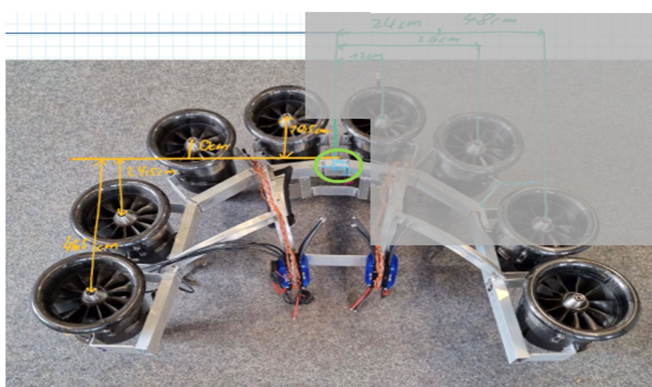
\includegraphics[width=0.75\textwidth, keepaspectratio]{lan4.png}
        \caption[FlyingSuit - wirksame Hebelarme bei der Torsion (Abbildungsverzeichnis)]{FlyingSuit - wirksame Hebelarme bei der Torsion}
        %\footcite{Rechter Teil des Bildes: Praktikum Schwingbruchgefaehrdete Bauteile sicher dimensionieren und betreiben
        %}
        
        \label{fig:lan4}
    \end{center}
\end{figure}

\clearpage
\subsubsection{Testaufbau}
Auch wenn es langfristig das Ziel ist, Messungen bei realen Testflügen durchzuführen und die Messtechnik eben dafür ausgelegt wurde,
ist es zunächst wichtig anfängliche Kalibreirungen und Tests, in einer definierten Umgebung abzuhalten.
In der Werkstatt von LandurisStudios besteht die Möglichkeit einen selbstentwickelten Teststand zu benutzen.
Dieser ermöglicht theoretisch Lasten bis zum Materialversagen zu simulieren und eignet sich besonders für statische Versuche.
Explorative dynamische Test können in sehr begrenztem Umfang ebenfalls erprobt werden.   Wie der Abbildung zu entnehmen, werden die Triebwerke durch Holzplatten ersetzt,
welche wiederum jeweils über einen Flaschenzug mit einem Gewicht verbunden sind. Dadurch können die Schubkräfte theoretisch beliebig experimentell simuliert werden.
Am Boden ist das Fluggestell, über den vorderen und den hinteren Aufnahmepunkt, fest verankert. Sind die simulierten Schubkräfte also größer als die notwendigen 8,4Kg,
um das Gestell auszugleichen, wird der Überschuss auf die Seilkräfte aufgeteilt und kann dort gemessen werden.
Die real vorgefundenen Gewichte hatten eine Masse von ca. 4.0Kg +/- 0.15Kg, was sowohl durch eine Zugwaage, als auch einen eigenen Kraftaufnehmer überprüft wurde.
Abzüglich der Gestell-masse, wird somit ein ca. 23.6Kg schwerer Pilot (ohne Akkus) dargestellt. Entsprechend können alle im weiteren Verlauf des Berichts durchgeführten Tests,
nur eine erste Abschätzung der realen Größenverhältnisse abbilden, wobei komplexere Bauteilparameter außer Acht gelassen werden.
\begin{figure}[htbp]
    \begin{center}
        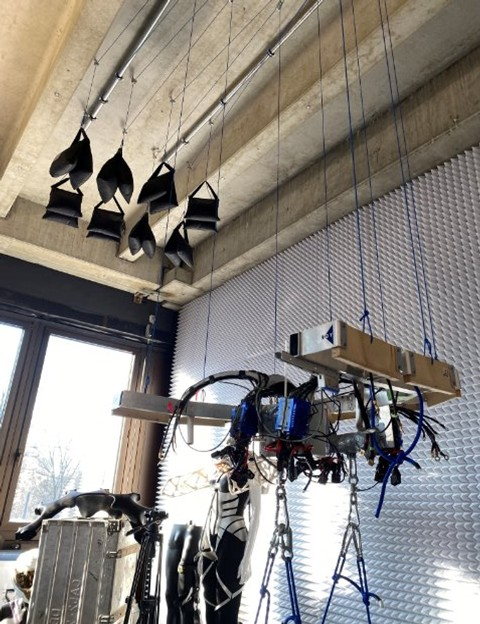
\includegraphics[width=0.5\textwidth, keepaspectratio]{lan5.jpg}
        \caption[Testaufbau - Gestell eingespannt (Abbildungsverzeichnis)]{Testaufbau - Gestell eingespannt}
        %\footcite{Rechter Teil des Bildes: Praktikum Schwingbruchgefaehrdete Bauteile sicher dimensionieren und betreiben
        %}
        
        \label{fig:lan5}
    \end{center}
\end{figure}

\subsubsection{Messaufbau}
Der Messaufbau besteht aus mehreren Komponenten, beginnend bei der Messbox mit dem Datenlogger, welche provisorisch frontal am Gestell befestigt wird.
Für die drei beschriebenen Testszenarien werden im einfachsten Fall, alle vier differentiellen Eingänge benötigt.
An Channel 1 und Channel 2 werden je ein 200Kg-1.4mV/V Kraftaufnehmer angeschlossen.
Diese werden zwischen den am Boden verankerten Seilen und den Aufnahmepunkten am Gestell mit Ringmuttern befestigt, um entsprechend die Zugkräfte aufzunehmen. 
\begin{figure}[htbp]
    \centering
    \begin{minipage}{0.48\textwidth}
        \centering
        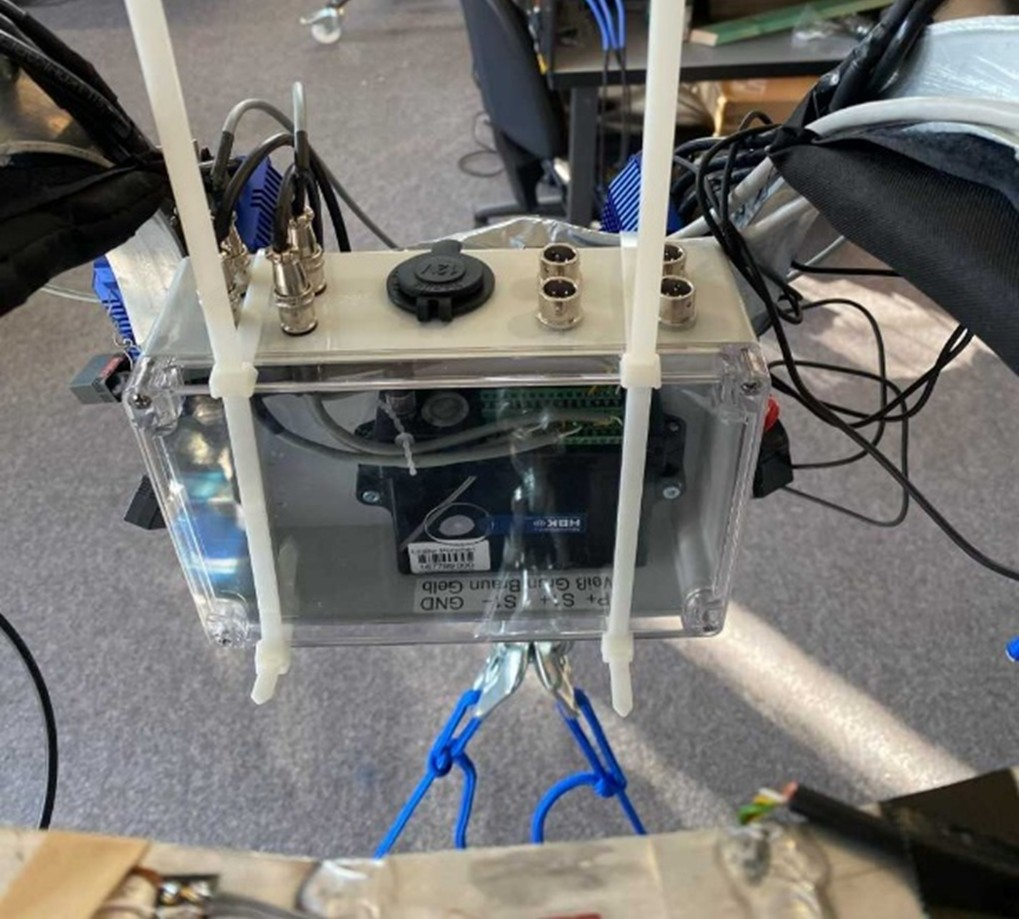
\includegraphics[width=\textwidth]{lan6.jpg}
        \caption[Messbox befestigt am Rahmen (Abbildungsverzeichnis)]{Messbox befestigt am Rahmen}
        
        \label{fig:lan6}
    \end{minipage}
    \hfill
    \begin{minipage}{0.48\textwidth}
        \centering
        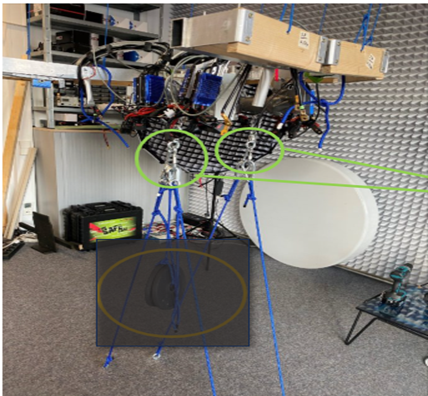
\includegraphics[width=\textwidth]{lan7.png}
        \caption[Kraftaufnehmer an den Aufnahmepunkten (Abbildungsverzeichnis)]{Kraftaufnehmer an den Aufnahmepunkten}
        
        \label{fig:lan7}
    \end{minipage}
\end{figure}

Für den Biegeversuch werden zwei 120 Ohm DMS benötigt, welche wie zuvor beschrieben hinten mittig platziert werden.
Wichtig zu erwähnen ist, das sämtliche folgende Montageschritte im nicht eingespannten, also unbelasteten Zustand, ohne simulierter Triebwerkskräfte, vorgenommen werden müssen.
Die DMS werden gemäß der verwendeten Halbbrücke und zu messenden Biegung, jeweils zentral auf der Ober- und der Unterseite des Rechteckquerschnittes platziert.

\begin{figure}[htbp]
    \begin{center}
        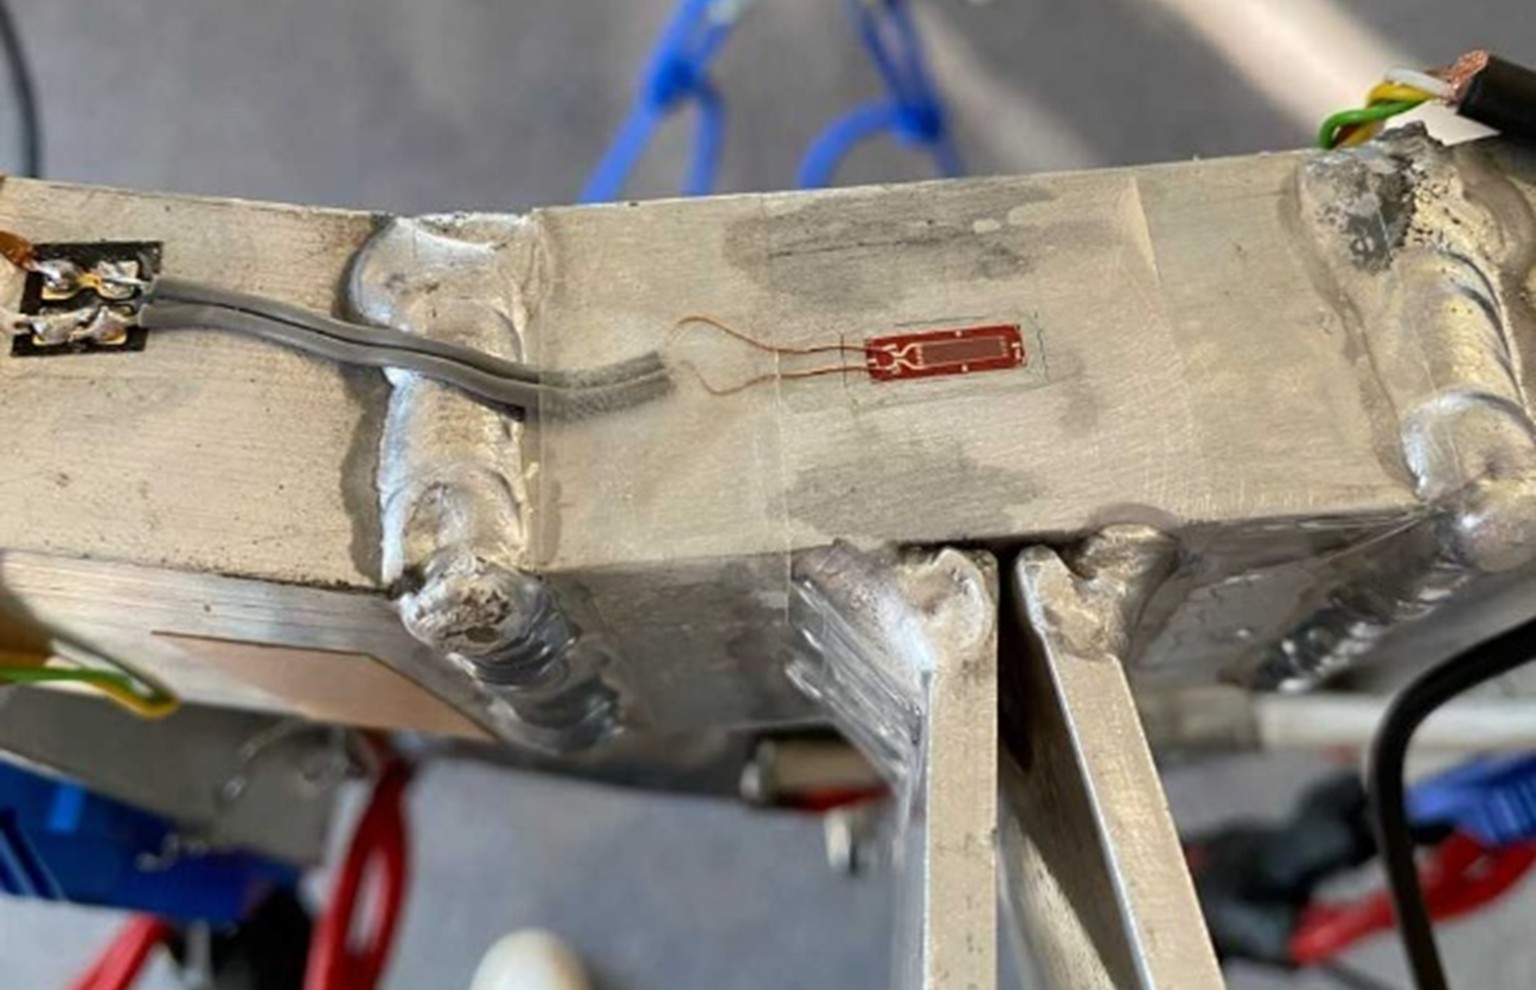
\includegraphics[width=0.5\textwidth, keepaspectratio]{lan8.jpg}
        \caption[Biegungs-DMS Fluggestell (Abbildungsverzeichnis)]{Biegungs-DMS Fluggestell}
        %\footcite{Rechter Teil des Bildes: Praktikum Schwingbruchgefaehrdete Bauteile sicher dimensionieren und betreiben
        %}
        
        \label{fig:lan8}
    \end{center}
\end{figure}


Vor dem Aufkleben ist es essentiell die Oberfläche anzurauen und mit Ethyl- Alkohol gründlich zu reinigen. Zudem sind Lötstützpunkte anzubringen.
Die DMS werden wie aus Kap 3 ersichtlich wird, untereinander, sowie mit dem vier- adrigen Kabel, welches auf die Brückenergänzugsplatine führt, verlötet. 


Der Torsionsversuch benötigt lediglich einen speziellen 120 Ohm Torsions DMS, da dieser zwei Messgitter beeinhaltet.
Der Aufbau ist dabei „Pfeilförmig“ mit zwei 45° Komponenten, da so die maximalen Schubdehnungen im Querschnitt erfasst werden.
Es ist anzumerken, dass aufgrund einer Fehlannahme, der DMS zu weit am Rand platziert wurde.
Um die Schubdehnungen/-spannungen ideal erfassen zu können, ist dieser ebenfalls zentral und horizontal, im Querschnitt, aufzukleben.
In der Abbildung wurde dies grün markiert. Die Grundsätzliche Montage erfolgt analog den Biegungs- DMS, jedoch ist bei der Verschaltung zu beachten,
dass nun lediglich drei statt vier Kabel vom DMS wegführen. Diese sind gemäß \ref{ch:systemaufbau} 3 zu einer sinnvollen Brückenschaltung zu verbinden.  

\begin{figure}[htbp]
    \centering
    \begin{minipage}{0.48\textwidth}
        \centering
        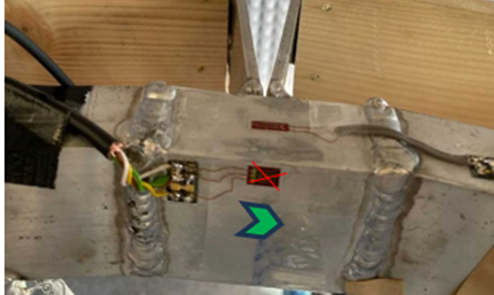
\includegraphics[width=\textwidth]{lan9.png}
        \caption[Torsions- DMS; in Grün die ideale Befestigungsstelle (Abbildungsverzeichnis)]{Torsions- DMS; in Grün die ideale Befestigungsstelle}
        
        \label{fig:lan9}
    \end{minipage}
    \hfill
    \begin{minipage}{0.48\textwidth}
        \centering
        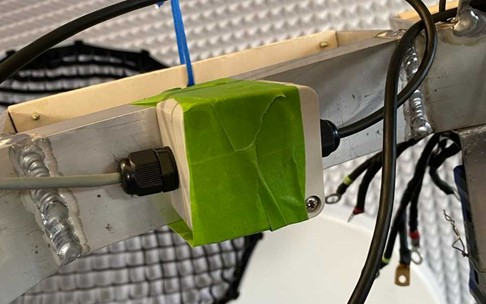
\includegraphics[width=\textwidth]{lan10.jpg}
        \caption[Platine für Halbbrückenergänzung am Gestell (Abbildungsverzeichnis)]{Platine für Halbbrückenergänzung am Gestell}
        
        \label{fig:lan10}
    \end{minipage}
\end{figure}

\clearpage
\subsection{Kalkulation/Geometrische Kalibrierung}
\label{sec:geo}
Die Zugkräfte bei Kräftegleichgewicht:

\begin{equation}
F_{\text{Zug}} = \frac{\text{Körpergewicht} + (\text{Anzahl Akkus} \times 2 \text{ kg je Akku}) + 1 \text{ kg Messbox}}{2}
\end{equation}

Für die Seilkräfte im Testaufbau:

\begin{equation}
F_{\text{Seil}} = \frac{(\text{Simulierter Schub Triebwerk} \times \text{Anzahl Triebwerke}) - 8,4 \text{ kg Gestell} - 1 \text{ kg Messbox}}{2}
\end{equation}

Mit den gegebenen Werten:

\begin{equation}
F_{\text{Seil}} = \frac{(4 \text{ kg} \times 8) - 8,4 \text{ kg} - 1 \text{ kg}}{2}
\end{equation}

\begin{equation}
F_{\text{Seil}} = \frac{32 \text{ kg} - 9,4 \text{ kg}}{2} = \frac{22,6 \text{ kg}}{2} = 11,3 \text{ kg}
\end{equation}

Umrechnung in Newton:

\begin{equation}
F_{\text{Seil}} = 11,3 \text{ kg} \times 9,81 \text{ N/kg} = 110,85 \text{ N}
\end{equation}

Im Testaufbau stellt sich automatisch ein Kräftegleichgewicht ein, da der Überschuss an simulierter Triebwerksleitung direkt durch die Seile aufgenommen werden. 

Zur Abschätzung der Biegung und Torsion an einem Rechteckholquerschnitt wurden folgende Formeln verwendet. Die eingesetzten Zahlenwerte entsprechen den gemessenen realen Werten am Testaufbau.

\textbf{Biegung:}

Simulierte Kraft je Triebwerk gemittelt:

\begin{equation}
F_{\text{Triebwerk}} = \frac{\sum (\text{Masse Gewichte} \cdot g)}{\text{Anzahl Gewichte}}
= \frac{32,17\,\text{kg} \times 9,81\,\text{N/kg}}{8} = 39,449\,\text{N}
\end{equation}

Maximales Biegemoment am Messpunkt in Abhängigkeit der Hebelarme:

\begin{equation}
M_{\text{max}} = 2 \cdot F_{\text{Triebwerk}} \cdot (l_1 + l_2 + l_3 + l_4)
\end{equation}

\begin{equation}
M_{\text{max}} = 2 \cdot 39,449\,\text{N} \cdot (120\,\text{mm} + 360\,\text{mm} + 2 \times 480\,\text{mm}) = 113613\,\text{Nmm}
\end{equation}

Flächenträgheitsmoment am Rechteckholquerschnitt:

\begin{equation}
I = \frac{b h^3 - b_i h_i^3}{12}
\end{equation}

\begin{equation}
I = \frac{25\,\text{mm} \cdot 50^3\,\text{mm}^3 - 21\,\text{mm} \cdot 46^3\,\text{mm}^3}{12} = 90078,67\,\text{mm}^4
\end{equation}

Maximale Biegespannung:

\begin{equation}
\delta_{\text{max}} = \frac{M_{\text{max}}}{I} \cdot \frac{h}{2}
\end{equation}

\begin{equation}
\delta_{\text{max}} = \frac{113613\,\text{Nmm}}{90078,67\,\text{mm}^4} \cdot 25\,\text{mm} = 31,532\,\text{N/mm}^2
\end{equation}

Dehnung aus Spannung und Elastizitätsmodul für Aluminium:

\begin{equation}
\varepsilon = \frac{\delta}{E} = \frac{31,532\,\text{N/mm}^2}{70000\,\text{N/mm}^2} = 0,45 \times 10^{-3} = 450\,\mu\text{m/m}
\end{equation}

Sensitivität berechnet in Abhängigkeit der DMS-Parameter und Halbbrückenkonfiguration:

\begin{equation}
\frac{U_B}{U_{\text{Ext}}} = \frac{N}{4} \cdot k \cdot \varepsilon = \frac{1}{2} \cdot 2,1 \cdot 0,45 \times 10^{-3} = 0,4725\,\text{mV/V}
\end{equation}

Brückenspannung:

\begin{equation}
U_B = U_{\text{Ext}} \cdot 0,4725\,\text{mV/V} = 1,936\,\text{V}
\end{equation}

\textbf{Torsion:}

Torsionsmoment um Querachse des Gestells:

\begin{equation}
M_{\text{Torsion}} = F \sum l_{\text{rechtsdrehend}} - F \sum l_{\text{linksdrehend}}
\end{equation}

\begin{equation}
M_{\text{Torsion}} = 2 \cdot 39,449\,\text{N} \cdot (245\,\text{mm} + 465\,\text{mm}) - 2 \cdot 39,449\,\text{N} \cdot 105\,\text{mm} = 47734,5\,\text{Nmm}
\end{equation}

Widerstandsmoment des Querschnitts:

\begin{equation}
J_{\text{polar}} = \frac{b h^3}{3} \left( 1 - \left( \frac{h_{\text{innen}}}{h} \right)^3 \right)
\end{equation}

\begin{equation}
J_{\text{polar}} = \frac{25\,\text{mm} \cdot 50^3\,\text{mm}^3}{3} \left( 1 - \left( \frac{46\,\text{mm}}{50\,\text{mm}} \right)^3 \right) = 230533,33\,\text{mm}^4
\end{equation}

Torsionsspannung im Abstand \( r \) zur Mittelachse:

\begin{equation}
\tau_{\text{Torsion}} = \frac{M_{\text{Torsion}} \cdot r}{J}
\end{equation}

\begin{equation}
\tau_{\text{Torsion}} = \frac{25\,\text{mm} \cdot 47734,5\,\text{Nmm}}{230533,33\,\text{mm}^4} = 5,177\,\text{N/mm}^2
\end{equation}

Schubdehnung:

\begin{equation}
\gamma = \frac{\tau_{\text{Torsion}}}{G} = \frac{5,177\,\text{N/mm}^2}{26000\,\text{N/mm}^2} = 199\,\mu\text{m/m}
\end{equation}

Gemessene Dehnung im DMS:

\begin{equation}
\varepsilon = \frac{\tau_{\text{Torsion}}}{E} = 74\,\mu\text{m/m}
\end{equation}

Sensitivität in Abhängigkeit der DMS-Parameter, zwei aktive Messgitter:

\begin{equation}
\frac{U_B}{U_{\text{Ext}}} = \frac{N}{4} \cdot k \cdot \varepsilon = \frac{1}{2} \cdot 2,06 \cdot 0,074 \times 10^{-3} = 0,0762\,\text{mV/V}
\end{equation}

Brückenspannung:

\begin{equation}
U_B = U_{\text{Ext}} \cdot 0,0762\,\text{mV/V} = 0,312\,\text{V}
\end{equation}



\section{Durchführung der Tests}
\subsection{Kraftaufnehmer}
Zu Beginn des Tests sind die beiden Kraftaufnehmer entsprechend ihren Herstellerangaben in der Software zu Kalibrieren.
Bei 200kg maximal zulässiger Last besitzen diese eine Sensitivität von 1.4mV/V.
Multipliziert mit der Versorgungsspannung von 4.096 V ergibt sich ein Messbereich von 5,344V bzw. 9,76V in den Einstellungen.
Experimentell wurde die Funktionstüchtigkeit der Kraftaufnehmer, durch Probemessungen definierter Gewichte, sowie dem Vergleich mit analogen Messvorrichtungen bestätigt. 
Durch die Rechnungen wurde eine gemessene Last je Kraftaufnehmer, von ca. 11,3 kg erwartet.
Zunächst wurde das Gestell mit den in der Beschreibung des Testaufbaus genannten Gewichten statisch belastet.
Durch unterschiedlich stark gespannte Seile des Testaufbaus, kam es hierbei zu deutlichen Abweichungen, sodass das eingespannte Gestell manuell ausgerichtet werden musste.
Auch wenn hierbei darauf geachtet wurde, den Aufbau so gerade wie möglich auszurichten, um eine ungefähr gleiche Lastverteilung zu erhalten, ist es nicht auszuschließen,
dass ein frei hängender Testaufbau hiervon abweichen könnte. Eine gleichmäßige Lastverteilung der Aufnahmepunkte zwischen Anzug und Gestell, ist damit nicht einwandfrei nachgewiesen. Die in Abbildung \ref{fig:lan11} zusehenden Messwerte, stimmen jedoch weitestgehend mit der Theorie überein.

\begin{figure}[htbp]
    \begin{center}
        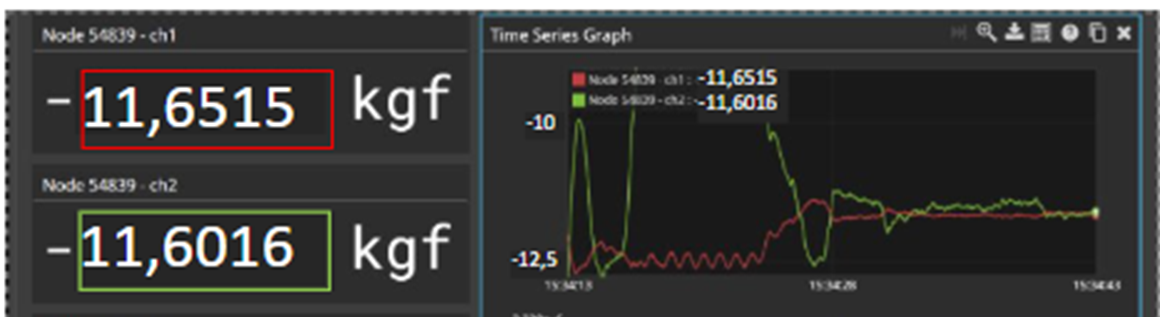
\includegraphics[width=1\textwidth, keepaspectratio]{lan11.png}
        \caption[Messung Kraftaufnehmer (Abbildungsverzeichnis)]{Messung Kraftaufnehmer}
        %\footcite{Rechter Teil des Bildes: Praktikum Schwingbruchgefaehrdete Bauteile sicher dimensionieren und betreiben
        %}
        
        \label{fig:lan11}
    \end{center}
\end{figure}

Im weiteren Verlauf wurde versucht neben dem statischen Test, auch erste dynamische Belastung zu simulieren.
Ziel hierbei war es zum einen die Darstellungsmöglichkeiten der Software näher kennenzulernen, als auch das tatsächliche Verhalten einer Steuereingabe am Gestell zu analysieren. 

Dabei wurden bekannte Gewichte abwechselnd an unterschiedliche Seiten des Gestells gehangen und auf Kommando losgelassen, siehe Abbildung \ref{fig:lan12}.

\begin{figure}[htbp]
    \begin{center}
        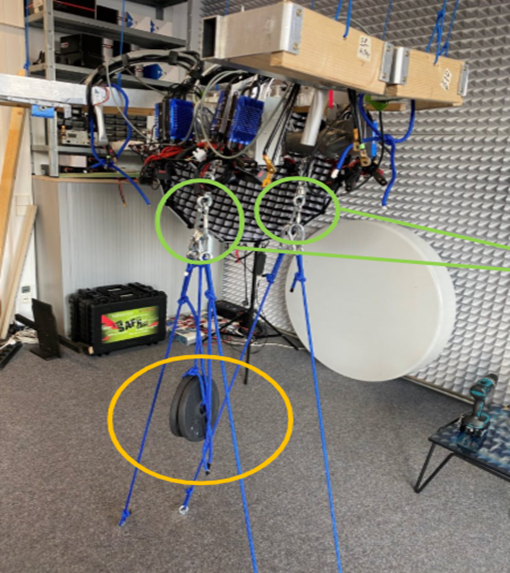
\includegraphics[width=0.5\textwidth, keepaspectratio]{lan12.png}
        \caption[Kraftaufnehmer Gewichte (Abbildungsverzeichnis)]{Kraftaufnehmer Gewichte}
        %\footcite{Rechter Teil des Bildes: Praktikum Schwingbruchgefaehrdete Bauteile sicher dimensionieren und betreiben
        %}
        
        \label{fig:lan12}
    \end{center}
\end{figure}

Der Zeitpunkt des einhängen und der Verlauf des einpendeln um eine neue Gleichgewichtslage, konnte dabei graphisch verfolgt werden.
Als praktikabel erwies es sich, Zeitabschnitte von 30 Sekunden zu plotten und als CSV- Datei für eine spätere Auswertung zu speichern.
Die oberflächlich betrachtet saubersten Graphen- Verläufe, konnten bei einer Abtastfrequenz von 128Hz erzielt werden, siehe Abbildung \ref{fig:lan13}.

\begin{figure}[htbp]
    \begin{center}
        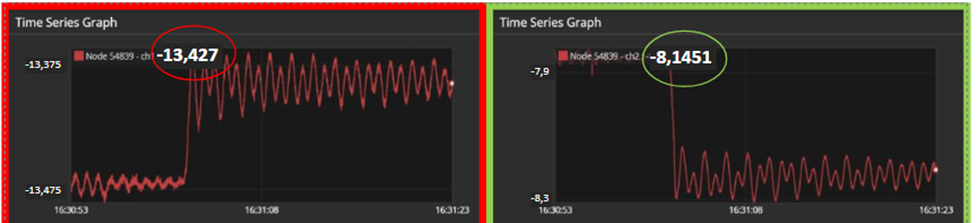
\includegraphics[width=1\textwidth, keepaspectratio]{lan13.png}
        \caption[Graphenverlauf Kraftaufnehmer (Abbildungsverzeichnis)]{Graphenverlauf Kraftaufnehmer}
        %\footcite{Rechter Teil des Bildes: Praktikum Schwingbruchgefaehrdete Bauteile sicher dimensionieren und betreiben
        %}
        
        \label{fig:lan13}
    \end{center}
\end{figure}

\subsection{Biegebeanspruchung}
Auch beim Test der Biegebeanspruchung muss vor Anfang der Messungen eine Kalibrierung stattfinden.
Die grundsätzliche Funktionsfähigkeit der Messbox, im Zusammenspiel mit Dehnungsmesstreifen, wurde bereits in einem Vorherigen Abschnitt am Biegebalken nachgewiesen.
Speziell zu Vorbereitung dieses Versuchs, wurde die interne Shunt- Kalibrierung durch eine Testmessreihe, ebenfalls am Biegebalken geprüft, sodass diese verwendet werden konnte.
In Betrachtung des Testaufbaus und der Messaufgabe, schien die Shunt- Kalibrierung als die praktikabelste, da sich die experimentelle Bestimmung schwierig gestaltet hätte, siehe Abbildung \ref{fig:shuntcal}. 
\begin{figure}[htbp]
    \begin{center}
        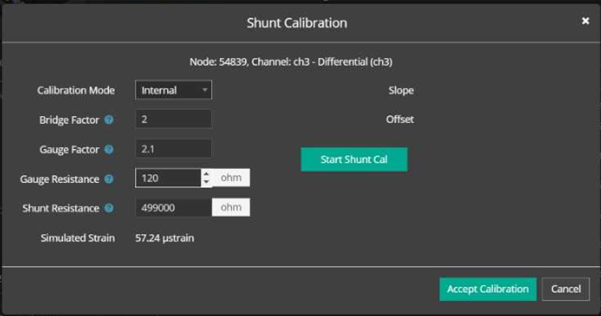
\includegraphics[width=0.5\textwidth, keepaspectratio]{shuntcal.png}
        \caption[Shuntkalibrierungseinstellungen (Abbildungsverzeichnis)]{Shuntkalibrierungseinstellungen}
        %\footcite{Rechter Teil des Bildes: Praktikum Schwingbruchgefaehrdete Bauteile sicher dimensionieren und betreiben
        %}
        
        \label{fig:shuntcal}
    \end{center}
\end{figure}


Um einen ungefähren Messbereich der zu erwartenden Biegespannung bzw. gemessen Biegedehnung, zu erhalten, kann die unter Kapitel \ref{sec:geo} durchgeführte Berechnung herangezogen werden.
Es ist anzumerken, dass die errechneten Werte relativ grobe Abschätzungen der erwarteten realen Werte darstellen,
da weder exakte Material-Parameter vorliegen noch die Versteifungen berücksichtigt wurden. Analog zum Zugversuch wurden zunächst statische Messungen vorgenommen,
um anschließend erste dynamische Versuche durchzuführen. Dazu wurden erneut Lasten als Störung des ursprünglichen Gleichgewichtszustandes in das System gegeben.

\begin{figure}[htbp]
    \begin{center}
        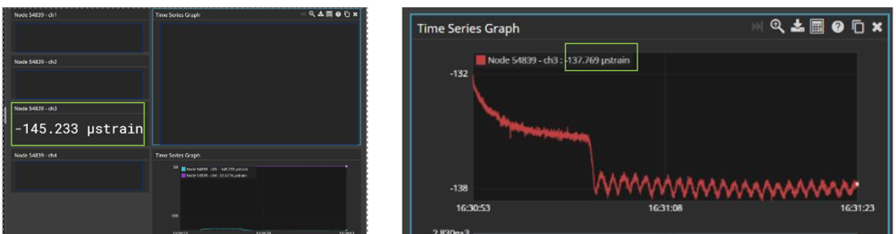
\includegraphics[width=1\textwidth, keepaspectratio]{mess1.png}
        \caption[Dynamische Messung (Abbildungsverzeichnis)]{Dynamische Messung}
        %\footcite{Rechter Teil des Bildes: Praktikum Schwingbruchgefaehrdete Bauteile sicher dimensionieren und betreiben
        %}
        
        \label{fig:mess1}
    \end{center}
\end{figure}


Die linke Seite von Abbildung \ref{fig:mess1} zeigt die statisch gemessene Biegedehnung im statischen Zustand. Der Wert stimmt dabei nicht mit der errechneten Dehnung von $450\,\mu\text{m/m}$ ein,
ist jedoch ungefähr im gleichen Bereich. Rechts in Abbildung \ref{fig:mess1} ist exemplarisch eine Belastung mit einer 5 kg Masse an der Rückseite des Gestells zu sehen.
Die tatsächliche Aussagekraft dieses Tests ist allerdings eingeschränkt. Mechanisch betrachtet findet, aufgrund der losen Lagerung der Gewichte im Testaufbau,
lediglich eine Umverteilung der Kräfte statt. Die in den Halteseilen aufgenommene Kraft wird hierbei durch Gewichtskraft ersetzt. Dennoch kann gezeigt werden,
dass die Darstellung der Belastungen über der Zeit, eindeutig gemessen werden kann.


\subsection{Torsionsbeanspruchung}
Das Vorgehen bei der Ermittlung der Torsionsbeanspruchung ist im Grunde analog zum Biegeversuch.
Bei der Shunt- Kalibrierung muss lediglich der leicht andere Gauge- Faktor von 2.06 beachtet werden.
Für einen Vergleich der erwarteten mit den tatsächlichen Messwerten, ist erneut die rechnerische Abschätzung hinzuzuziehen. 


Links auf Abbildung \ref{fig:mess2} ist auch hier die gemessene statische Torsionsdehnung im DMS zu sehen.
Vergleicht man dies mit den errechneten $74\,\mu\text{m/m}$, sind die Abweichungen nochmals kleiner als bei der Biegung.
Ergänzend hinzuzufügen ist, dass aufgrund der nicht zentralen Platzierung des Torsions- DMS, die gemessene Dehnung geringer ist als die maximal vorliegende.
Rechts in Abbildung \ref{fig:mess2}zeigt den Verlauf beim dynamischen Versuch mit einer 5 kg Masse hinten. Auch hier ist er tatsächliche mechanische Erkenntnisgewinn in Frage zu stellen.
Dennoch ist das Ziel einer Darstellung des Belastungsverlauf erfüllt. 
\begin{figure}[htbp]
    \begin{center}
        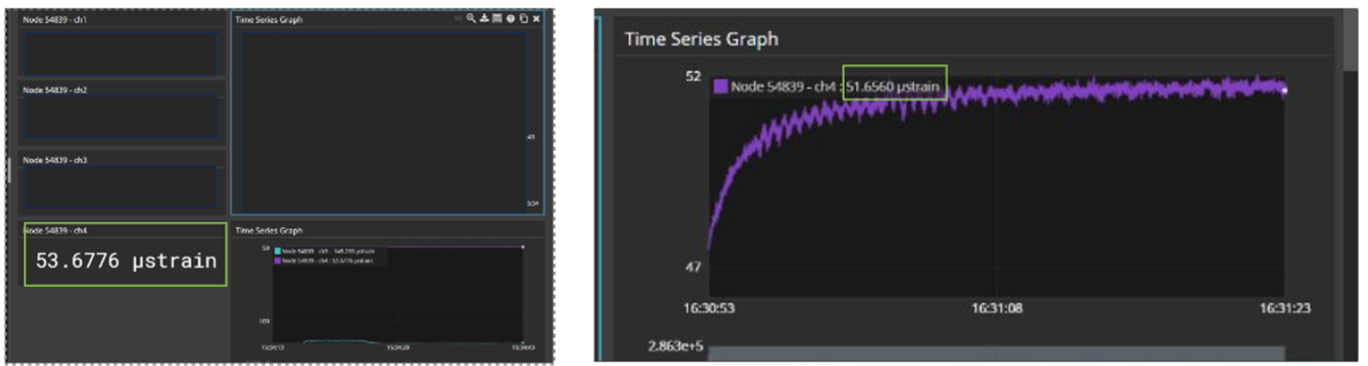
\includegraphics[width=1\textwidth, keepaspectratio]{mess2.png}
        \caption[Torsionsbeanspruchung(Abbildungsverzeichnis)]{Torsionsbeanspruchung}
        %\footcite{Rechter Teil des Bildes: Praktikum Schwingbruchgefaehrdete Bauteile sicher dimensionieren und betreiben
        %}
        
        \label{fig:mess2}
    \end{center}
\end{figure}